% Chapter Template

\chapter{Ensayos y resultados} % Main chapter title

\label{Chapter4} % Change X to a consecutive number; for referencing this chapter elsewhere, use \ref{ChapterX}

%----------------------------------------------------------------------------------------
%	SECTION 1
%----------------------------------------------------------------------------------------

\section{Proceso de desarrollo y aseguramiento de calidad}
\label{sec:pruebasHW}

...

\section{Prototipos de los diferentes modulos}
\label{sec:pruebasHW}


\subsection{Prototipo de funcionalidad de medición de temperatura y humedad}

Para el desarrollo de este prototipo se utilizaron el framework ESP-IDF y como la librería de código de ESP-IDF Components Lib para la gestión del DHT11. A continuación se puede apreciar el conexionado del prototipo.

\begin{center}
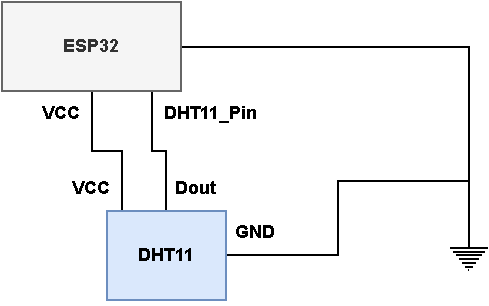
\includegraphics[scale=0.75]{conexionado_dht11}
\end{center}

De acuerdo al pinout de ESP32 [ref] se configuraron los pines de acuerdo a la tabla a continuación. 

\begin{center}

\begin{tabular}{|c |c |c |c|} 
 \hline
 Logic Name & Pin GPIO  \\ [0.5ex] 
 \hline
 Pin DHT11  & 2  \\ [1ex] 
 \hline
\end{tabular}


\end{center}
\subsection{Prototipo de funcionalidad de medicion de presion}
Para el desarrollo de este prototipo se utilizaron el framework ESP-IDF y como la librería de código de ESP-IDF Components Lib para la gestión del BMP280. A continuación se puede apreciar el conexionado del prototipo.

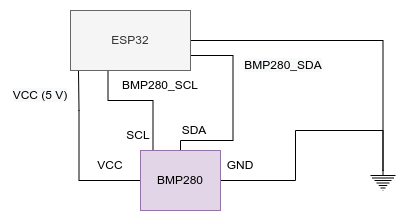
\includegraphics[scale=0.75]{conexionado_bmp280}
De acuerdo al pinout de ESP32 [ref] se configuraron los pines de acuerdo a la tabla a continuación. 

\begin{center}

\begin{tabular}{|c |c |c |c|} 
 \hline
 Logic Name & Pin GPIO  \\ [0.5ex] 
 \hline
 BMP SDA & 18 \\
 BMP280 SCL & 19  \\ [1ex] 
 \hline
\end{tabular}



\end{center}
\subsection{Prototipo de funcionalidad de medición de valor de luminosidad}
Para el desarrollo de este prototipo se utilizó el siguiente conexionado y la librería de código ADC provista por ESP-IDF. 

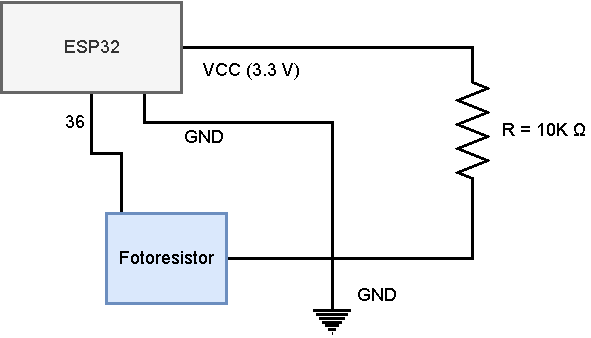
\includegraphics[scale=0.75]{conexionado_fotoresistor}

De acuerdo al pinout de ESP32 [ref] se configuraron los pines de acuerdo a la tabla a continuación.

\begin{center}

\begin{tabular}{|c |c |c |} 
 \hline
 Logic Name & Pin ADC & Pin GPIO \\ [0.5ex] 
 \hline
 ADC_Fot_pin & channel 0 - unit 2 & 4\\ [1ex] 

 \hline
\end{tabular}


\end{center}
\subsection{Prototipo de funcionalidad de obtencion de valores analogicos del joystick}
Para el desarrollo de este prototipo se utilizó el siguiente conexionado y la librería de código ADC provista por ESP-IDF. 



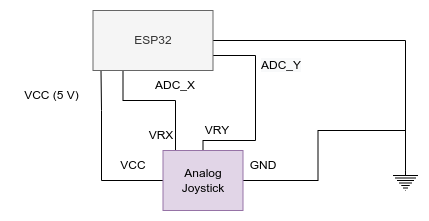
\includegraphics[scale=0.75]{conexionado_joystick}

De acuerdo al pinout de ESP32 [ref] se configuraron los pines de acuerdo a la tabla a continuación.

\begin{center}

\begin{tabular}{|c |c |c |} 
 \hline
 Logic Name & Pin ADC & Pin GPIO \\ [0.5ex] 
 \hline
 ADC_X & channel 1 - unit 2 & 0 \\ 
 ADC_Y & channel 7 - unit 1 & 35 \\ [1ex] 

 \hline
\end{tabular}

\end{center}

\subsection{Prototipo de funcionalidad de presentación de display}
 

\subsection{Prototipo de funcionalidad de control de motores DC}


...

\section{Tests de los diferentes modulos}
\label{sec:pruebasHW}

...

\section{Tests del producto final}
\label{sec:pruebasHW}

...

\section{Reportes de testing}
\label{sec:pruebasHW}

...

\section{Verificacion y validacion del producto}
\label{sec:pruebasHW}

...

\section{Documentacion del producto }
\label{sec:pruebasHW}

...



